\part{Partial-Fractions}
\lecture{Partial Fractions}{Partial-Fractions}
\section{Partial Fractions}


\title{Partial Fractions}
\subtitle{It Is Not Just For Integration Any More}
\date{13 November 2013}

\begin{frame}
  \titlepage
\end{frame}

\begin{frame}
  \frametitle{Outline}
  \tableofcontents[ currentsection ]
\end{frame}


\subsection{The Project and the Test}

\begin{frame}{The Project and the Test}
  \centerline{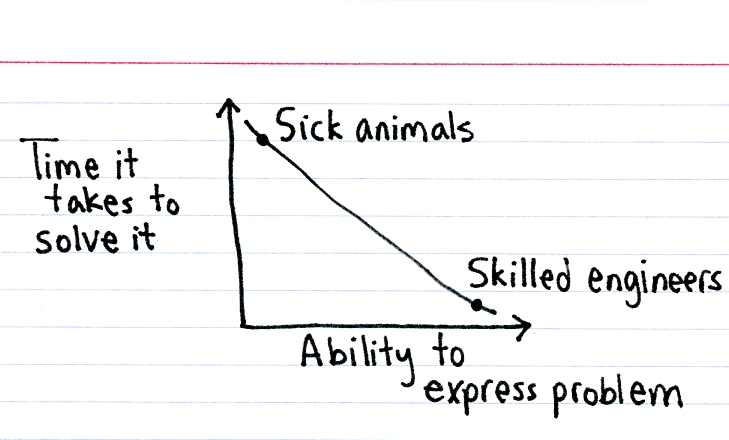
\includegraphics[width=5cm]{img/skilledEngineers}}

  {\tiny
    (from
    \url{http://thisisindexed.com/2013/10/just-tell-me-whats-the-matter/})
  }

  It is coming up!
\end{frame}
\subsection{Partial Fractions}


\iftoggle{clicker}{%
\begin{frame}
  \frametitle{Clicker Quiz}

   \ifnum\value{clickerQuiz}=1{%
     What is the common denominator for
     \begin{eqnarray*}
       \frac{3}{7} + \frac{2}{3}?
     \end{eqnarray*}
     \begin{tabular}{ll}
       A: & $3$  \\ [12pt]
       B: & $7$  \\ [12pt]
       C: & $14$ \\ [12pt]
       D: & $21$ \\ [12pt]
     \end{tabular}

     \vfill
   }\fi

   \ifnum\value{clickerQuiz}=2{%
     What is the common denominator for
     \begin{eqnarray*}
       \frac{-1}{5} + \frac{7}{8}?
     \end{eqnarray*}
     \begin{tabular}{ll}
       A: & $5$  \\ [12pt]
       B: & $8$  \\ [12pt]
       C: & $40$ \\ [12pt]
       D: & $45$ \\ [12pt]
     \end{tabular}


   \vfill
   }\fi

  \ifnum\value{clickerQuiz}=3{%
    What is the common denominator for
     \begin{eqnarray*}
       \frac{-3}{7} + \frac{7}{8}?
     \end{eqnarray*}
     \begin{tabular}{ll}
       A: & $7$  \\ [12pt]
       B: & $8$  \\ [12pt]
       C: & $56$ \\ [12pt]
       D: & $24$ \\ [12pt]
     \end{tabular}

  \vfill
 }\fi
\end{frame}
}


\begin{frame}
  \frametitle{Partial Fractions}

  Appendix PF in your book.

  \uncover<2->
  {
    \begin{eqnarray*}
      \frac{6}{x-3} - \frac{4}{x-2} & = & 
      \uncover<3->
      {
        \frac{6(x-2)}{(x-2)(x-3)} - \frac{4(x-3)}{(x-2)(x-3)}\\
        & = & \frac{2x}{x^2-5x+6}
      }
    \end{eqnarray*}
  }

\end{frame}


\begin{frame}
  \frametitle{Integration}

  \begin{eqnarray*}
    \int \frac{2x}{x^2-5x+6} ~ dx & = & \int \frac{6}{x-3} - \frac{4}{x-2} ~ dx \\
    & = & 6\ln(x-3) - 4\ln(x-2) + C.
  \end{eqnarray*}

  \uncover<2->
  {
    Question: How do we do this backwards?

    Answer: Expand in terms of unknown coefficients and ``do the algebra.''
  }

\end{frame}


\begin{frame}
  \frametitle{The Idea}

  We have the ratio of two polynomials, $\frac{p(x)}{q(x)}$:
  \begin{itemize}
  \item The degree of $p(x)$ is less than the degree of $q(x)$.
  \item Factor $q(x)$.
  \item Write out a general expansion in terms of the factors.
  \item Solve for unknown constants.
  \end{itemize}

\end{frame}

\subsection{Examples}

\begin{frame}
  \frametitle{Example}

  \begin{eqnarray*}
    \frac{2x}{x^2-5x+6} & = & 
    \uncover<2->
    {
      \frac{2x}{(x-3)(x-2)}, \\
      & = & \frac{a}{x-3} + \frac{b}{x-2}.
    }
  \end{eqnarray*}

  \uncover<3->
  {
    Multiply both sides by $(x-3)(x-2)$:
    \begin{eqnarray*}
      \lefteqn{\frac{2x}{(x-3)(x-2)} \cdot (x-3)(x-2)  } \\
      & = & \lp \frac{a}{x-3} + \frac{b}{x-2} \rp \cdot (x-3)(x-2), \\
      \uncover<4->
      {
        & = &  \frac{a}{x-3} \cdot (x-3)(x-2) + \frac{b}{x-2} \cdot (x-3)(x-2), \\
      }
      \uncover<5->
      {
        2x & = & a (x-2) + b(x-3)
      }
    \end{eqnarray*}
  }


\end{frame}


\begin{frame}
  \frametitle{Solve for the Constants}
  \vspace*{-1em}
  We have:
  \begin{eqnarray*}
    2x & = & a (x-2) + b(x-3).
  \end{eqnarray*}

  Let $x=2$:
  \begin{eqnarray*}
    2(2) & = & a ((2)-2) + b((2)-3) \\
    \Rightarrow 4 & = & -b.
  \end{eqnarray*}

  Let $x=3$:
  \begin{eqnarray*}
    2(3) & = & a ((3)-2) + b((3)-3) \\
    \Rightarrow 6 & = & a.
  \end{eqnarray*}

  \uncover<2->
  {
    Substitute back into the original expansion:
    \begin{eqnarray*}
      \frac{2x}{x^2-5x+6} & = & \frac{6}{x-3} - \frac{4}{x-2}.
    \end{eqnarray*}
  }

\end{frame}


\begin{frame}
  \frametitle{Example}

  \begin{eqnarray*}
    \frac{5x}{x^2+4x-32} & = & \uncover<2->{ \frac{5x}{(x-4)(x+8) }} \\
    \uncover<3->{ & = & \frac{a}{x-4} + \frac{b}{x+8} } \\
    \uncover<4->{ 5x & = & a (x+8) + b (x-4).}
  \end{eqnarray*}

  \uncover<5->
  {
    Let $x=-8$:
    \begin{eqnarray*}
      -40 & = & -12b, \\
      b & = & \frac{10}{3}.
    \end{eqnarray*}

    Let $x=4$:
    \begin{eqnarray*}
      20 & = & 12a, \\
      a  & = & \frac{5}{3}.
    \end{eqnarray*}

  }


\end{frame}


\begin{frame}

    Substitute back in to get
    \begin{eqnarray*}
    \frac{5x}{x^2+4x-32} & = & \frac{5/3}{x-4} + \frac{10/3}{x+8} 
    \end{eqnarray*}


\end{frame}


\iftoggle{clicker}{%
\begin{frame}
  \frametitle{Clicker Quiz}

   \ifnum\value{clickerQuiz}=1{%
     What is the common denominator for
     \begin{eqnarray*}
       \frac{3}{x-5} + \frac{8}{(x-5)^2}?
     \end{eqnarray*}
     \begin{tabular}{ll}
       A: & $x-5$ \\ [12pt]
       B: & $(x-5)^2$ \\ [12pt]
       C: & $\ln(x-5)$ 
     \end{tabular}

     \vfill
   }\fi

   \ifnum\value{clickerQuiz}=2{%
     What is the common denominator for
     \begin{eqnarray*}
       \frac{-1}{x+7} + \frac{12}{(x+7)^2}?
     \end{eqnarray*}
     \begin{tabular}{ll}
       A: & $x+7$ \\ [12pt]
       B: & $(x+7)^2$ \\ [12pt]
       C: & $\ln(x+7)$ 
     \end{tabular}


   \vfill
   }\fi

  \ifnum\value{clickerQuiz}=3{%
     What is the common denominator for
     \begin{eqnarray*}
       \frac{-4}{x+9} + \frac{12}{(x+9)^2}?
     \end{eqnarray*}
     \begin{tabular}{ll}
       A: & $x+9$ \\ [12pt]
       B: & $(x+9)^2$ \\ [12pt]
       C: & $\ln(x+9)$
     \end{tabular}
 
  \vfill
 }\fi
\end{frame}
}


\begin{frame}
  \frametitle{Quadratic Terms}

  Note that
  \begin{eqnarray*}
    \frac{2}{x+2} + \frac{4}{(x+2)^2} & = & \frac{2(x+2)+4}{(x+2)^2}, \\
    & = & \frac{2x+8}{x^2+4x+4}.
  \end{eqnarray*}

\end{frame}


\begin{frame}
  \frametitle{Example}

  \begin{eqnarray*}
    \frac{2x+8}{x^2+4x+4} & = & \uncover<2->{ \frac{2x+8}{(x+2)^2}} \\
    \uncover<3->{ & = & \frac{a}{x+2} + \frac{b}{(x+2)^2} } \\
    \uncover<4->{ 2x+8 & = & a (x+2) + b.}
  \end{eqnarray*}

  \uncover<5->
  {
    Let $x=-2$:
    \begin{eqnarray*}
      4 & = & b.
    \end{eqnarray*}

    Let $x=0$:
    \begin{eqnarray*}
      8 & = & 2a+b, \\
      a  & = & 2.
    \end{eqnarray*}

  }


\end{frame}


\begin{frame}

    Substitute back in to get
    \begin{eqnarray*}
    \frac{2x+8}{x^2+4x+4} & = & \frac{2}{x+2} + \frac{4}{(x+2)^2} 
    \end{eqnarray*}


\end{frame}


\begin{frame}
  \frametitle{Example}

  \begin{eqnarray*}
    \frac{3x+1}{x^2+6x+9} & = & \uncover<2->{ \frac{3x+1}{(x+3)^2}} \\
    \uncover<3->{ & = & \frac{a}{x+3} + \frac{b}{(x+3)^2} } \\
    \uncover<4->{ 3x+1 & = & a (x+3) + b.}
  \end{eqnarray*}

  \uncover<5->
  {
    Let $x=-3$:
    \begin{eqnarray*}
      -8 & = & b.
    \end{eqnarray*}

    Let $x=0$:
    \begin{eqnarray*}
      1 & = & 3a+b, \\
      a  & = & 3.
    \end{eqnarray*}

  }


\end{frame}


\begin{frame}

    Substitute back in to get
    \begin{eqnarray*}
    \frac{3x+1}{x^2+6x+9} & = & \frac{3}{x+3} - \frac{8}{(x+3)^2} 
    \end{eqnarray*}


\end{frame}


\begin{frame}
  \frametitle{Example}

  \begin{eqnarray*}
    \frac{4x^2+1}{x^3-3x^2-4x} & = & \uncover<2->{ \frac{4x^2+1}{x(x-4)(x+1)}} \\
    \uncover<3->{ & = & \frac{a}{x} + \frac{b}{x-4} + \frac{c}{x+1} } \\
    \uncover<4->{ 4x^2+1 & = & a (x-4)(x+1) + bx(x+1) + cx(x-4).}
  \end{eqnarray*}

  \uncover<5->
  {
    Let $x=4$:
    \begin{eqnarray*}
      b & = & \frac{13}{4}.
    \end{eqnarray*}

    Let $x=-1$:
    \begin{eqnarray*}
      c & = & 1.
    \end{eqnarray*}

    Let $x=0$:
    \begin{eqnarray*}
      a & = & \frac{-1}{4}.
    \end{eqnarray*}

  }


\end{frame}


\begin{frame}

    Substitute back in to get
    \begin{eqnarray*}
    \frac{4x^2+1}{x^3-3x^2-4x} & = & \frac{-1/4}{x} + \frac{13/4}{x-4} + \frac{1}{x+1}.
    \end{eqnarray*}


\end{frame}


\begin{frame}
  \frametitle{Example}

  \begin{eqnarray*}
    \frac{2x^2+3x-2}{x^3-3x+2} & = & \uncover<2->{ \frac{2x^2+3x-2}{(x-1)^2(x+2)}} \\
    \uncover<3->{ & = & \frac{a}{x-1} + \frac{b}{(x-1)^2} + \frac{c}{x+2} } \\
    \uncover<4->{ 2x^2+3x-2 & = & a (x-1)(x+2) + b(x+2) + c(x-1)^2.}
  \end{eqnarray*}

  \uncover<5->
  {
    Let $x=1$:
    \begin{eqnarray*}
      b & = & 1.
    \end{eqnarray*}

    Let $x=-2$:
    \begin{eqnarray*}
      c & = & 0.
    \end{eqnarray*}

    Let $x=0$:
    \begin{eqnarray*}
      a & = & 2.
    \end{eqnarray*}

  }


\end{frame}


\begin{frame}

    Substitute back in to get
    \begin{eqnarray*}
    \frac{2x^2+3x-2}{x^3-3x+2} & = & \frac{2}{x-1} + \frac{1}{(x-1)^2}.
    \end{eqnarray*}


\end{frame}


\begin{frame}
  \frametitle{More Quadratics}

  \begin{eqnarray*}
    \frac{x+3}{x^2+x+4} - \frac{1}{x-2} & = & 
    \frac{(x+3)(x-2)}{(x-2)(x^2+x+4)} - \frac{x^2+x+4}{(x-2)(x^2+x+4)}, \\
    & = & \frac{x^2+x-6-(x^2+x+4)}{(x-2)(x^2+x+4)}, \\
    & = & \frac{-10}{(x-2)(x^2+x+4)}. \\
  \end{eqnarray*}

\end{frame}

\begin{frame}
  \frametitle{Working It Backwards}
  
  Given
  \begin{eqnarray*}
    \frac{-10}{(x-2)(x^2+x+4)} & = & \frac{a}{x-2} + \frac{bx+c}{x^2+x+4}, \\
    \Rightarrow -10 & = & a(x^2+x+4) + (bx+c)(x-2).
  \end{eqnarray*}

  \uncover<2->
  {
    Let $x=2$:
    \begin{eqnarray*}
      a & = & -1.
    \end{eqnarray*}

    %%%%%%%%%%%%%%%%%%%%
    Let $x=0$:
    \begin{eqnarray*}
      c & = & 3.
    \end{eqnarray*}
 
    Let $x=1$:
    \begin{eqnarray*}
      b & = & 1.
    \end{eqnarray*}

    Substitute back in to get
    \begin{eqnarray*}
     \frac{-10}{(x-2)(x^2+x+4)}= \frac{-1}{x-2} + \frac{x+3}{x^2+x+4}. 
  \end{eqnarray*}

    %Match the polynomial terms:
    %\begin{eqnarray*}
    %  -10 & = & -(x^2+x+4) + (bx+c)(x-2), \\
    %  -10 & = & -x^2 - x - 4 + bx^2 - 2bx + cx - 2c, \\
    %  \Rightarrow b & = & 1, \\
    %  c & = & 3.
    %\end{eqnarray*}
  }

\end{frame}


\begin{frame}
  \frametitle{General Forms}

  \begin{eqnarray*}
    \frac{1}{x^3+1} & = & \frac{1}{(x+1)(x^2-x+1)}= \frac{a}{x+1} + \frac{bx+c}{x^2-x+1}.
  \end{eqnarray*}

  \begin{eqnarray*}
    \frac{5}{(x^2+4)(x^2-x+10)} & = & \frac{ax+b}{x^2+4} + \frac{cx+d}{x^2-x+10}.
  \end{eqnarray*}

  \begin{eqnarray*}
    \frac{18}{(x-1)(x+2)(x+3)} & = & \frac{a}{x-1} + \frac{b}{x+2} + \frac{c}{x+3}.
  \end{eqnarray*}


  \begin{eqnarray*}
    \frac{4}{x^2(3x^2+2)} & = & \frac{a}{x} + \frac{b}{x^2} + \frac{cx+d}{3x^2+2}.
  \end{eqnarray*}

  \begin{eqnarray*}
    \frac{4}{x^2(3x^2-2)} & = & \frac{a}{x} + \frac{b}{x^2} + \frac{c}{x+\sqrt{\frac{2}{3}}} + \frac{d}{x-\sqrt{\frac{2}{3}}}.
  \end{eqnarray*}

  
\end{frame}



% LocalWords:  Clarkson pausesection hideothersubsections
